\documentclass[pdf]{beamer}
\usepackage{alltt}
\usepackage{array}
\usepackage{lmodern}
\usepackage[T1]{fontenc}
\usepackage[utf8]{inputenc}
%\usepackage{beamerthemesplit}
\usepackage{pgf}
\usepackage{tikz}
\usepackage{xkeyval}
\usepackage{hevea}
\usepackage{mathpartir}

\usetikzlibrary{shadows}
\usetikzlibrary{arrows}

\setbeamercovered{transparent}

\definecolor{lightgreen}{HTML}{95F4A2}
\definecolor{lightred}{HTML}{F4959D}
\definecolor{darkgreen}{HTML}{01802A}
\usetheme{frama-c}

\setbeamerfont{smaller}{size=\footnotesize}

\pgfdeclareimage[width=\textwidth,interpolate=true]{gwhy}{gwhy}

\title[Frama-C training session]{Jessie Plugin and ACSL Specifications}
\author[Virgile Prevosto]{Virgile Prevosto}
\date[03-31-2009]{March 31, 2009}
\institute[CEA List]{CEA List}

\AtBeginSection[]{
\begin{frame}
 \frametitle{}
 \tableofcontents[currentsection]
 \end{frame}
 }

% Exemples de verification:
% - moyenne ?
% - listes ou tableaux ?
% Choses à faire passer:
% - les différentes composantes d'une spec, invariant (et variant) de
% boucle
% - comment lire la fenetre gwhy
% - les debordements
% - "collaboration" analyse de valeur jessie
% - les alias et les preconditions a respecter
% - terminaison et ensures \false

%\newcommand<>{\onlyverbatim}[1]{\verb!#1!}

\newcommand{\vfilll}{\vspace*{0pt plus1filll}}

\newcommand{\launch}[2]{%
\only<beamer>{%
  \leavevmode%
  \pdfstartlink user {%
    /Subtype /Link
    /A <</S /Launch
    /F (#1)
       >>
       }%
  #2%
  \pdfendlink%
}
\only<handout>{#2}
}

\begin{document}
\begin{frame}
\titlepage
\end{frame}

\begin{frame}{outline}
\tableofcontents
\end{frame}

\section{Jessie Usage}

\begin{frame}{What is Jessie?}
\begin{itemize}
\item<+-> Hoare-logic based plugin, developed at INRIA Saclay.
\item<+-> Input: a program and a specification
\item<+-> Jessie generates \alert{verification conditions}
\item<+-> Use of \alert{Automated Theorem Provers} to discharge the VCs
\item<+-> If all VCs are proved, \alert{the program is correct} with respect
  to the specification
\item<+->Otherwise: need to investigate why the proof fails
\begin{itemize}
\item<+-> Fix bug in the code
\item<+-> Adds additional annotations to help ATP
\item<+-> Interactive Proof (Coq/Isabelle)
\end{itemize}
\end{itemize}
\end{frame}

\begin{frame}{What is Jessie Useful for?}
\begin{block}{Usage}
\begin{itemize}
\item<+-> Proof of functional properties of the program
\item<+-> Modular verification (function per function)
\end{itemize}
\end{block}
\pause
\begin{block}{Limitations}
\begin{itemize}
\item<+->Cast between pointers and integers
\item<+->Limited support for union type
\item<+->Aliasing requires some care
\end{itemize}
\end{block}
\end{frame}

\begin{frame}[fragile]{From Frama-C to Theorem Provers}
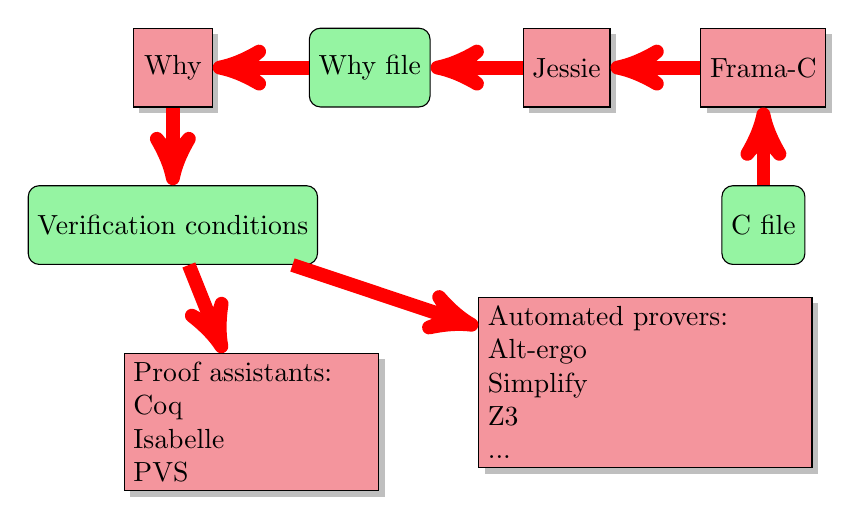
\begin{tikzpicture}[%
file/.style={minimum size=1cm,draw,rounded corners,fill=lightgreen},
arrow/.style={line width=5pt,draw=red,-stealth'},
tool/.style={minimum size=1cm,draw,fill=lightred,drop shadow}
]
\node[style=file] (c file) at (9.5,9) {C file};
\node[style=tool] (frama-c) at (9.5,11){Frama-C};
\node[style=tool] (jessie) at (7,11) {Jessie};
\node[style=file] (why file) at (4.5,11) {Why file};
\node[style=tool] (why) at (2,11) {Why};
\node[style=file] (vc) at (2,9) {Verification conditions};
\node[style=tool] (atp) at (8,7)
  { \begin{minipage}{4cm}Automated provers:\newline Alt-ergo\newline Simplify\newline Z3\newline...\end{minipage}};
\node[style=tool] (pa) at (3,6.5) {\begin{minipage}{3cm}
    Proof assistants:\newline Coq\newline
    Isabelle\newline PVS\end{minipage}};
\path[style=arrow] (c file) -- (frama-c);
\path[style=arrow] (frama-c) -- (jessie);
\path[style=arrow] (jessie) -- (why file);
\path[style=arrow] (why file) -- (why);
\path[style=arrow] (why) -- (vc);
\path[style=arrow] (vc) -- (atp);
\path[style=arrow] (vc) -- (pa);
\end{tikzpicture}
\end{frame}

\begin{frame}[fragile]{A first example}
  \begin{block}{Check safety of a function}
    \begin{itemize}
      \item Pointer accesses
      \item Arithmetic overflow
      \item Division
    \end{itemize}
  \end{block}

  \input{mean_orig.pp}
\end{frame}

\begin{frame}<handout>{A first specification}
  \input{mean_res.pp}
\end{frame}

\section{Function Contracts}

\begin{frame}
  \frametitle{Behavior of a function}
  \begin{itemize}
  \item Functional specification
  \item<2->Pre-conditions (\texttt{requires})
  \item<3->Post-conditions (\texttt{ensures})
  \end{itemize}

  \begin{block}{Example}
    \input{mean_spec_orig.pp}
  \end{block}
\end{frame}

\begin{frame}
  \setbeamercovered{invisible}
  \frametitle{Side effects}
  \begin{block}{The specification:}%
  \input{meansig.pp}
  \end{block}
\only<handout>{
  \vfill
  \begin{block}{An admissible implementation:}
    \begin{overprint}
      \only<handout:1>{\input{4bad1.pp}}%
      \only<handout:2>{\input{4bad2.pp}}%
      \only<handout:3>{\input{4good.pp}}
    \end{overprint}
  \end{block}
}
\end{frame}

 \begin{frame}<handout>
   \frametitle{Termination}
     \begin{itemize}
     \item<1> Post condition true \emph{when the function exits normally.}
     \item<3> By default, a function always terminates...
     \item<4> ... as long as its pre-condition holds.
     \end{itemize}
   \input{mean_terminates.pp}
 \end{frame}

\section{Generating Proof Obligations}

\begin{frame}{Hoare logic}
\begin{itemize}
\item Introduced by Floyd and Hoare (70s)
\item Hoare triple: $\{P\}s\{Q\}$, meaning: \emph{If $P$ holds, then
  $Q$ will hold after the execution of statement $s$}
\item Deduction rules on Hoare triples: \emph{Axiomatic semantic}
\end{itemize}
\end{frame}

\begin{frame}[fragile]{Some rule examples}
\begin{mathpar}
\inferrule{ }{\{P\}\textrm{\ttfamily\upshape{}\{\}}\{P\}} \and
\inferrule{ P \Rightarrow P' \and \{P'\}\textrm{\ttfamily\upshape{}s}\{Q'\} \and
            Q' \Rightarrow Q}
          {\{P\}\textrm{\ttfamily\upshape{}s}\{Q\}}
\and
\inferrule{\{P\}\textrm{\ttfamily\upshape{}s\_{}1}\{R\} \\ \{R\}\textrm{\ttfamily\upshape{}s\_{}2}\{Q\}}
{\{P\}\textrm{\ttfamily\upshape{}s\_{}1;s\_{}2}\{Q\}}
\and
\inferrule{e~\textrm{evaluates without error}}
          {\{P[x\leftarrow e]\}\textrm{\ttfamily\upshape{}x=e;}\{P\}} \and
\inferrule{\{P \wedge \textrm{\ttfamily\upshape{}e}\}\textrm{\ttfamily\upshape{}s\_{}1}\{Q\} \\
           \{P\wedge \textrm{\ttfamily\upshape{}!e}\}\textrm{\ttfamily\upshape{}s\_{}2}\{Q\}}
  {\{P\}\textrm{\ttfamily\upshape{}\textbf{\textcolor{red}{if}}~(e)~\{~s\_{}1~\}~\textbf{\textcolor{red}{else}}~\{~s\_{}2~\}}\{Q\}}
  \and
\inferrule{\{I\wedge \textrm{\ttfamily\upshape{}e}\}\textrm{\ttfamily\upshape{}s}\{I\}}
{\{I\}\textrm{\ttfamily\upshape{}\textbf{\textcolor{red}{while}}~(e)~\{~s~\}}\{I \wedge \textrm{\ttfamily\upshape{}!e}\}}
\end{mathpar}
\end{frame}

\begin{frame}{Weakest pre-condition}
\begin{itemize}
\item<+->Program seen as a \alert{predicate transformer}
\item<+->Given a function $s$, a pre-condition $Pre$ and a
  post-condition $Post$
\item<+->We start from $Post$ at the end of the function and go backwards
\item<+->At each step, we have a property $Q$ and a statement $s$, and
  compute the \emph{weakest pre-condition} $P$ such that $\{P\}s\{Q\}$
  is a valid Hoare triple.
\item<+->When we reach the beginning of the function with property
  $P$, we must prove $Pre\Rightarrow P$.
\end{itemize}
\end{frame}

\begin{frame}{Some rules}
\begin{itemize}
\item Assignment
\[
WP(\textrm{\ttfamily\upshape{}x=e},Q) = Q[x\leftarrow e]
\]
\item Sequence
\[
WP(\textrm{\ttfamily\upshape{}s\_{}1;s\_{}2},Q) = WP(\textrm{\ttfamily\upshape{}s\_{}1},WP(s_2;Q))
\]
\item Conditional
\[
\begin{array}{lc}
WP(\textrm{\ttfamily\upshape{}\textbf{\textcolor{red}{if}}~(e)~\{~s\_{}1~\}~\textbf{\textcolor{red}{else}}~\{~s\_{}2~\}},Q) & = \\
\hspace*{1cm}\textrm{\ttfamily\upshape{}e}\Rightarrow WP(\textrm{\ttfamily\upshape{}s\_{}1},Q) \wedge \textrm{\ttfamily\upshape{}!e}\Rightarrow
WP(\textrm{\ttfamily\upshape{}s\_{}2},Q)
\end{array}
\]
\item While
\[
\begin{array}{lc}
WP(\textrm{\ttfamily\upshape{}\textbf{\textcolor{red}{while}}~(e)~\{~s~\}},Q) & =  \\
\hspace*{1cm}I \wedge
 \forall\omega. I\Rightarrow(\textrm{\ttfamily\upshape{}e}\Rightarrow WP(\textrm{\ttfamily\upshape{}s},I) \wedge
                             \textrm{\ttfamily\upshape{}!e}\Rightarrow Q)
\end{array}
\]
\end{itemize}
\end{frame}

\begin{frame}[fragile]{Memory Model}
\begin{block}{Issue}
How can we represent memory operations (\verb|*x|,
\verb|a[i]=42|,\ldots) in the logic
\end{block}

\begin{itemize}
\item If too low-level (a big array of bytes), proof obligations are
  intractable.
\item If too abstract, some C constructions can not be represented
  (arbitrary pointer casts, aliasing)
\item Standard solution (Burstal-Bornat): replace struct's components
  by a function
\end{itemize}
\end{frame}

\begin{frame}{Aliasing}
\begin{block}{Issue}
The same memory location can be accessed through different means:
\input{alias.pp}
\end{block}
\begin{itemize}
\item Again, supposing that any two pointers can be aliases would lead
  to intractable proof obligations.
\item Memory is separated in disjoint regions
\item Some hypotheses are done (as additional pre-conditions)
\end{itemize}
\end{frame}

\begin{frame}<handout>{In practice}
\pgfuseimage{gwhy}
\end{frame}

\section{Advanced Specification}
\subsection{Example 1: Searching}
\begin{frame}{A concrete example}
\begin{block}{Informal spec}
\begin{itemize}
\item Input: a \alert{sorted} array and its length, an element to search.
\item Output: index of the element or \texttt{-1} if not found
\end{itemize}
\end{block}
\begin{block}{Implementation}
\input{find_array_orig.pp}
\end{block}
\end{frame}

\begin{frame}<handout>{Predicate definition}
\begin{block}{What does ``sorted'' mean?}
\begin{syntax}
  rel-op ::= "==" | "!=" | "<=" | ">=" | ">" | "<"
       \
  pred ::= "\true" | "\false" ;
       | term (rel-op term)+ ;               \hspace{-10mm} comparisons
       | id "(" term ("," term)* ")" ;       \hspace{-10mm} predicate application
       | "(" pred ")" ;                      \hspace{-10mm} parentheses
       | [ pred "&&" pred ] ;                \hspace{-10mm} conjunction
       | [ pred "||" pred ] ;                \hspace{-10mm} disjunction
       | [ pred "==>" pred ] ;               \hspace{-10mm} implication
       | pred "<==>" pred ;                  \hspace{-10mm} equivalence
       | "!" pred ;                          \hspace{-10mm} negation
       | pred "^^" pred ;                    \hspace{-10mm} exclusive or
       | [ term "?" pred ":" pred ] ;        \hspace{-10mm} ternary condition
       | [ pred "?" pred ":" pred ];
       | "\let" id "=" term ";" pred ;       \hspace{-10mm} local binding
       | { "\let" id "=" pred ";" pred };
       | [ "\forall" binders ";" ] ;
           [ integer-guards "==>" pred ];    \hspace{-10mm} univ. integer quantification
       | [ "\exists" binders ";" ];
           [ integer-guards "&&" pred ] ;    \hspace{-10mm} exist. integer quantification
       | [ { "\forall" binders ";" } ] ;
         [ { iterator-guard "==>" pred } ];  \hspace{-10mm} univ. iterator quantification
       | [ { "\exists" binders ";" } ];
         [ { iterator-guard "&&" pred } ] ;  \hspace{-10mm} exist. iterator quantification
       | [ { "\forall" binders ";" pred } ]; \hspace{-10mm} univ. quantification
       | [ { "\exists" binders ";" pred } ]; \hspace{-10mm} exist. quantification
       | id ":" pred ;                       \hspace{-10mm} syntactic naming
       | string ":" pred ;                   \hspace{-10mm} syntactic naming
       \
  [ integer-guards ] ::= [ interv  ("&&" interv)* ]
       \
  [ interv ]  ::= [ (term integer-guard-op)+ ] ;
                  [ id ] ;
                  [ (integer-guard-op term)+ ]
       \
  [ integer-guard-op ] ::= [ "<=" | "<" ]
       \
  [ { iterator-guard } ] ::= [ { id "(" term"," term ")" } ]
\end{syntax}

\end{block}
\begin{block}{ACSL predicates}
\begin{itemize}
\item Give a formal definition of the properties of objects
\item Can be used in annotations
\item Must be tied to a program point when performing a memory access
\item Some predicate can relate two or more program points (see after)
\end{itemize}
\end{block}
\end{frame}

\begin{frame}<handout>[fragile]{Function behaviors}

\verb+find_array+ has two distinct \alert{behaviors}, depending on
whether the query is in the array or not. This can be reflected in the
contract in the following way:

\input{find_array_contract.pp}
\end{frame}

\begin{frame}<handout>{Loop invariant}
\begin{block}{Role of the loop invariant}
\begin{itemize}
\item Must be inductive (if it holds at the beginning, then it holds
  at the end)
\item Capture the effects of one loop step
\item Represents the only things known at the exit of the loop
\item Must be strong enough to allow to derive the post-condition
\end{itemize}
\end{block}
\begin{block}{Example}
\input{find_array_invariant.pp}
\end{block}
\end{frame}

\begin{frame}<handout>{Loop variant}
\begin{block}{Total correctness}
\begin{itemize}
\item Needed for proving termination
\item Expression which strictly decreases at each step
\item And stay non-negative
\end{itemize}
\end{block}
\begin{block}{Example}
\input{find_array_variant.pp}
\end{block}
\end{frame}

\begin{frame}<handout>{Assertions}
\begin{block}{Usage}
\begin{itemize}
\item A property which must hold at a given point
\item Allows to guide the automated provers
\item Can be associated to a particular behavior
\end{itemize}
\end{block}
\begin{block}{Example}
\input{find_array_assertions.pp}
\end{block}
\end{frame}

\subsection{Example 2: Sorting}

\begin{frame}{An example}
  \begin{block}{Informal specification}
    \begin{itemize}
      \item Input: an array and its length
      \item Output: the array is sorted in ascending order
    \end{itemize}
  \end{block}
  \input{sort_array_orig.pp}
\end{frame}

\begin{frame}<handout>{Function Calls}
  \begin{itemize}
    \item Post-conditions and assigns are the only things that the
      caller knows when the callee returns
    \item Caller must fulfill the pre-condition of callee before the call
  \end{itemize}
\end{frame}

\begin{frame}<handout>
  \frametitle{Inductive Predicates}
    \begin{itemize}
    \item Case definition: $H_i \Rightarrow Pred$
    \item Horn clause: $Pred$ can only appear positively in $H_i$
      (ensures consistency)
    \item Smallest fixpoint: predicate holds iff one of the $H_i$ holds
    \end{itemize}
  \input{sort_inductive.pp}
\end{frame}
\end{document}

Local Variables:
mode: latex
ispell-local-dictionary: "english"
End:
